
\section{Introdução}

No trabalho, é realizada uma simulação de um processo de reação-difusão com
atividade catalítica a partir de modelos desenvolvidos em\cite{3}.

Esses sistemas de reação-difusão são sistemas que envolvem reagentes sendo
convertidos em produtos por uma reação química e transportados no espaço pela
difusão. Esse tipo de sistema é muito estudado em engenharia química, mas ocorre
frequentemente também em outras áreas\cite{4}.

A simulação do trabalho possui como objetivo, a reprodução de resultados já
alcançados por meio desses modelos e propiciar o aprendizado e desenvolvimento
desse método numérico de modelagem de sistemas reais.

Simulação é uma forma de modelagem utilizada na análise de sistemas complexos
que envolve, portanto, o desenvolvimento de um modelo matemático que, após a
prática de experimentações deste modelo , possibilita a obtenção de um histórico
de comportamento do sistema ao longo do tempo e de estatísticas desse
comportamento\cite{1}. A figura \ref{Figure-011-Simulacao} mostra a relação do
processo de simulação com a área de modelagem matemática de sistemas.

{ \centering
	\hfill \break
	\captionsetup{type=figure}
	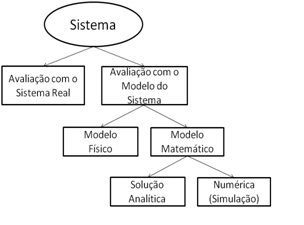
\includegraphics[width=\columnwidth]{./figures/011-Simulacao.jpg}
	\captionof{figure}{Simulação em Modelagem de Sistemas\cite{1}}
	\label{Figure-011-Simulacao}
}

O modelo matemático, por sua vez, pode ser definido como ``uma
representação, em termos matemáticos, do comportamento de objetos e dispositivos
reais''\cite{2} (tradução nossa). Esse modelo pode ser analítico ou de
simulação, que diferem pela natureza de suas soluções. Modelos analíticos
possuem como solução, uma equação fechada que descreve o comportamento do
sistema ao longo do tempo\cite{1}.

Modelos de simulação são solucionados por meio da execução de um programa que
gera amostras do comportamento do sistema, que permite realização de análises
do sistema\cite{1}. As etapas de desenvolvimento desse tipo de modelo é
descrita na figura \ref{Figure-012-EtapaSimulacao}.

O problema a ser tratado pela simulação é a análise comportamental da reação de
armadilhamento com desativação ao longo do tempo. Para uma formulação apropriada
deste problema e o posterior desenvolvimento de um modelo conceitual para tal
sistema, primeiro deve ser analisado o problema de forma mais simples, sem
desativação da armadilha, cujo modelo já possui solução analítica na
bibliografia. Esse modelo corresponde a uma versão discreta do modelo de
Smoluchowski\cite{5}.

{ \centering
	\hfill \break
	\captionsetup{type=figure}
	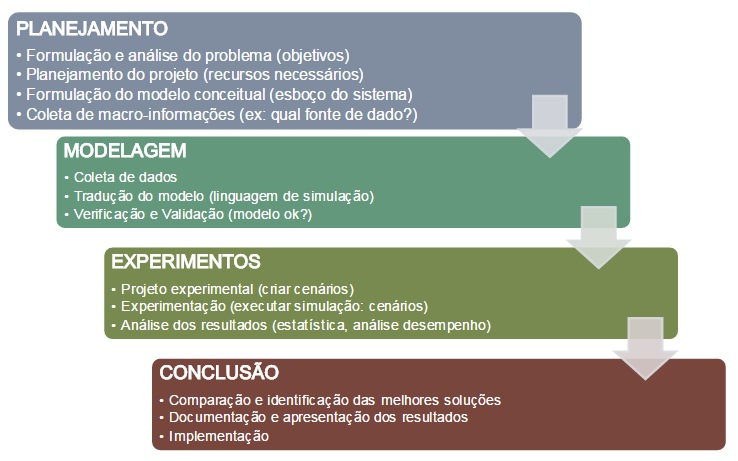
\includegraphics[width=\columnwidth]{./figures/012-EtapaSimulacao.jpg}
	\captionof{figure}{Etapas do processo de simulação\cite{1}}
	\label{Figure-012-EtapaSimulacao}
}
